\documentclass[12pt,a4paper,oneside]{book} % twoside for draf

%\usepackage{times}
\usepackage{graphicx}
\usepackage{subcaption}
\usepackage[utf8x]{vietnam}
\usepackage[english]{babel}
\selectlanguage{english}
\usepackage{mathptmx}	% same Time New Roma
%\renewcommand{\rmdefault}{phv} % Arial
%\renewcommand{\sfdefault}{phv} % Arial
\usepackage{url}

%link to part by click on contents region
\usepackage{hyperref}
\hypersetup{
    colorlinks,
    citecolor=black,
    filecolor=black,
    linkcolor=black,
    urlcolor=black
}

\usepackage{fancyhdr}
\usepackage{algorithm2e}
\usepackage{amsmath}
\usepackage{array,tabularx}
\usepackage{amsfonts}
\usepackage{amssymb}
\usepackage{cases}
\usepackage{tabularx}
\usepackage{adjustbox}
\usepackage{multirow}

\usepackage{bkthesis}

\usepackage{titlesec}

%\titleformat{\chapter}[display]
%  {\normalfont\bfseries}{}{0pt}{\Huge}

\usepackage{tikz}
\usetikzlibrary{shapes,arrows}

\newenvironment{conditions*}
  {\par\vspace{\abovedisplayskip}\noindent
   \tabularx{\columnwidth}{>{$}l<{$} @{${}:{}$} >{\raggedright\arraybackslash}X}}
  {\endtabularx\par\vspace{\belowdisplayskip}}

\tikzstyle{blank} = [text badly centered, node distance = 2cm, inner sep=0pt]
\tikzstyle{block} = [rectangle, draw, 
    text width=2em, text centered, minimum height=2em]
\tikzstyle{line} = [draw, -latex']

\newcolumntype{b}{>{\hsize=1.0\hsize}X}

\crname{THESIS PROPOSAL}
\ctname{Name of THESIS}
\cstuname{
	Students: \\
	\begin{tabular}{ l c }
	    Nguyễn Nguyên Phương & 1712726\\
		Nguyễn Đình Thắng & 1752048
	\end{tabular}
}


\csCouncil{Computer Science}
\csSupervise{Nguyễn An Khương}
\csReviewer{No name}
\cttime{12/2020}

\thesislayout

\begin{document}

\coverpage

\frontmatter

\begin{declaration}
We hereby undertake that this is our own research project under the guidance of Dr. Nguyen. Research content and results are truthful and have never been published before. The data used for the analysis and comments are collected by us from many different sources and will be clearly stated in the references.

In addition, we also use a number of reviews and figures of other authors and organizations. All have citations and origins.

If we detect any fraud, we take full responsibility for the content of our graduate internship. Ho Chi Minh City University of Technology is not related to the copyright and copyright infringement caused by us in the implementation process.

\end{declaration}
~

\begin{acknowledgments}

First and foremost, we would like to express our sincere gratitude to our advisor Dr. Nguyen for the support of our thesis proposal for his patience, enthusiasm, experience and knowledge. He shared his experience and knowledge which helps us in our research and how to provide a good thesis proposal.
\end{acknowledgments}
~

%
\begin{abstract}
Charts have been and always will be one of the most effective tools for demonstrating and sharing ideas among others. Besides text and images, drawing flow charts is the best way to give others a clearer path of the plan with the least amount of work. Nowadays, many meetings require a blackboard so everyone can express their thoughts on. This raised a problem with saving these drawings as a reference for future use since taking a picture of them will not solve the problem of re-editing these ideas and they need to be re-drawn to be suitable in professional documents. On the other hand, in order to digitalize the chart required to re-draw it using a computer or a special device like drawing boards and digital pens, which cost a lot and is not the most convenient tools to use.

Therefore, it is necessary to find a new way to convert the current hand-drawing charts into digital ones effortless, simplify the sharing process between users and be able to export them into another form like picture files (png, jpg), document files (pdf) or common diagram editing files (drawio). The application must be able to run on popular platforms and accessible by everyone.
\end{abstract}
 
\tableofcontents
%\listofsymbols
\listoftables
\listoffigures
%\listofalgorithms


\mainmatter

\fancypagestyle{plain}{%
\fancyhf{}
\fancyfoot[LE, RO]{\thepage}
\renewcommand{\headrulewidth}{0.0pt}
}

\pagestyle{fancy}
\renewcommand{\chaptermark}[1]{\markboth{\MakeUppercase{#1}}{}}
\fancyhf{}
\fancyhead[LE,RO]{\leftmark}
\fancyhead[RE,LO]{}
\fancyfoot[LE,RO]{\thepage}
\renewcommand{\footrulewidth}{0.4pt}

%\fancyhead{}  % Clears all page headers and footers
%\rhead{\thepage}  % Sets the right side header to show the page number
%\lhead{}  % Clears the left side page header
%\fancyfoot[positions]{footer}
%\renewcommand{\footrulewidth}{0.4pt}

%\pagestyle{fancy}  % Finally, use the "fancy" page style to implement the FancyHdr headers


\chapter{Introduction} \label{Introduction}
\minitoc

\section{Overview}

\subsection{Problem statements}

\subsubsection{HDWallet architect}

\subsubsection{Protocols}

\subsubsection{Algorithm}

\subsection{Explain why this thesis is chosen}

\section{Objectives}

\subsection{Aims}

\subsection{Practical benefits/application}

\section{Scope of the study}

\section{Tentative structure of the study}

\section{Tentative schedule}
\chapter{Background}
\label{chap:background}
	\textit{In this chapter, we introduce the foundation knowledge of the thesis, including the history and definition of Blockchain Technology, Cryptocurrency, 
	Hierarchical Deterministic Wallet (HD Wallet) and Cryptography}
\minitoc

\section{Blockchain Technology}

\subsection{History and Definition}

Blockchains are immutable digital ledger systems implemented in a distributed fashion (i.e., without a central repository) and usually without a central authority.
The definition of blockchain was introduced to the world by a person (or a group of people) under the name Satoshi Nakamoto on October 31, 2008. 
It was applied to enable the emergence of a "purely peer-to-peer (no financial institution or third party) electronic cash" named Bitcoin where transactions take place in a distributed system.
In fact, Satoshi did not invent blockchain, and Bitcoin blockchain is not the first chain that ever created. 
Back in 1991, cryptographers Stuart Haber and Scott Stornetta published a whitepaper "How to Time-Stamp a Digital Document" in the Journal of Cryptography. 
Their goal is to digital time-stamping of documents so that it is infeasible for a user either to back-date or to a forward-date digital document, even with the collusion of a time-stamping service. 
The technology is called a blockchain because the distributed electronic ledger stores items of data in time-stamped digital groups called blocks. Each block includes an alphanumeric code called a "hash" summing up its data. The hash of each completed block also appears in the next one in the chain, which means that to alter one block you would have to alter all the ones connected to it. These cryptographic dominos function together to protect against tampering or fraud.
Base on this theory, the longest-running blockchain, started in 1995, also by Haber and Stornetta, publishes the weekly summary hash value every week in the New York Times (\autoref{fig:first_blockchain}) and still running strong today. 

\begin{figure}[h!]
	\centering
	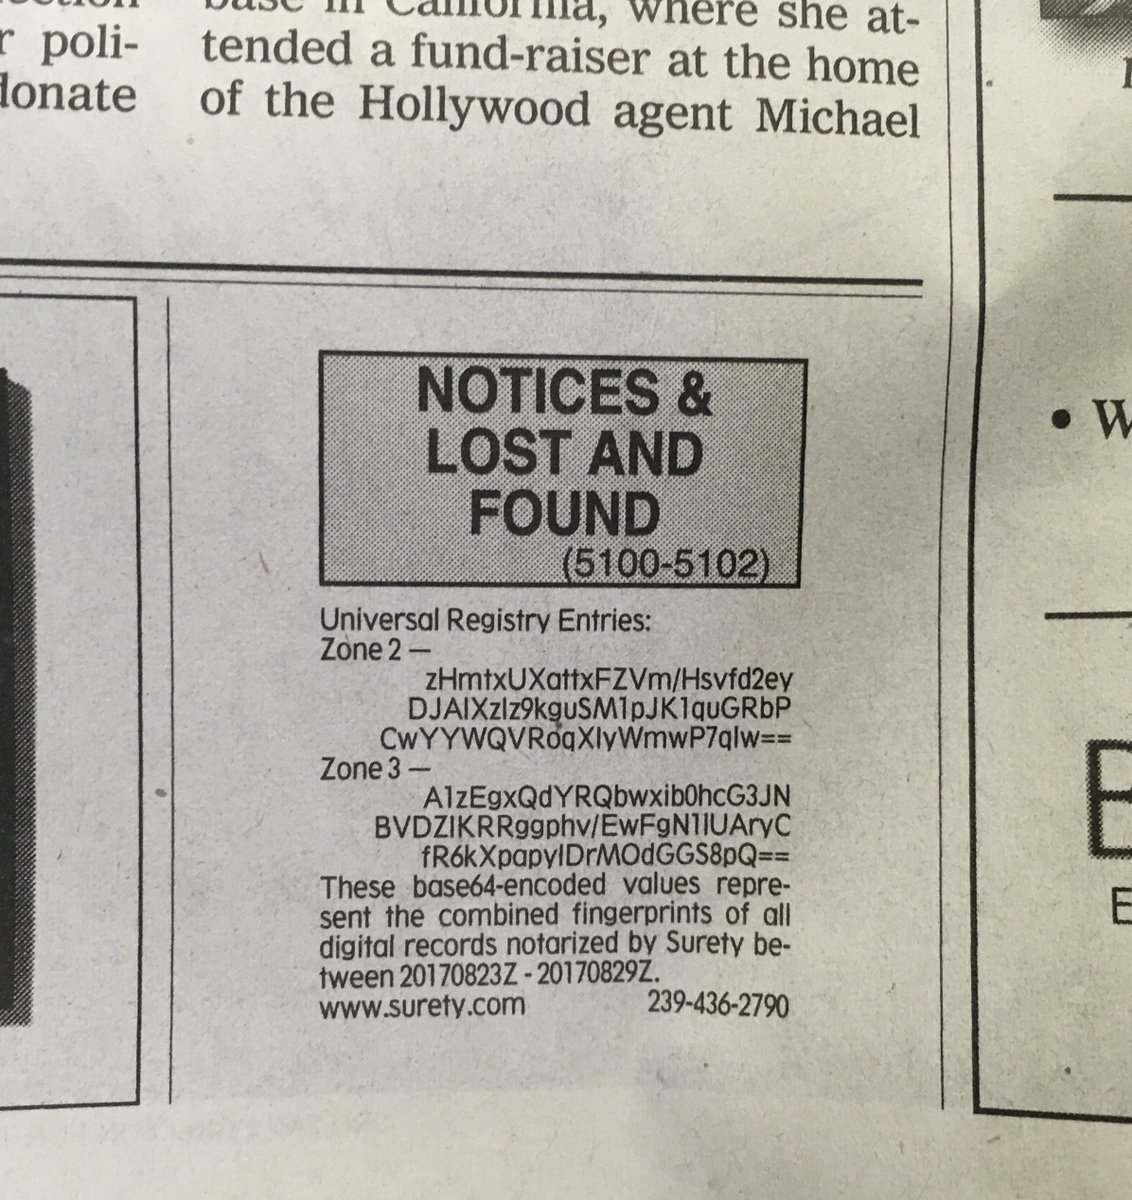
\includegraphics[width=.35\textwidth]{images/Widely_Witnessed_Values.jpg}
	\caption[Widely-Witnessed Values of Surety, a weekly summary (hash) of documents]{Weekly summary hash value in The New York Times}
	\label{fig:first_blockchain}
\end{figure}

% The math behind blockchain and its complex system architecture make it challenging to understand. 
But the word "blockchain" or "block" and "chain" wasn't use back then. 
Only it become known in Satoshi Nakamoto's Bitcoin paper in the term of "chain" of "blocks".
Later people combined the one-word "blockchain" in mainstream media publications such as Fortune, Forbes, and the Huffington Post as the technology gained greater interest and use. 
The comunity use that word for Nakamoto's invention.
Bound to emergence of Bitcoin and cryptocurrency, a concise description of blockchain technology is provided by NIST:

\begin{quote} 
	Blockchains are distributed digital ledgers of cryptographically signed transactions that are grouped into blocks. Each block is cryptographically linked to the previous one (making it tamper evident) after validation and undergoing a consensus decision. As new blocks are added, older blocks become more difficult to modify (creating tamper resistance). New blocks are replicated across copies of the ledger within the network, and any conflicts are resolved automatically using established rules.
\end{quote}

Blockchain technology comes handy in a wide range of areas - both ​financial and non-financial​. 
Non-Financial application opportunities are endless. 
We can envision putting proof of the existence of all legal documents, health records, and loyalty payments in the music industry, notary, private securities and marriage licenses in the blockchain. 
By storing the fingerprint of the digital asset instead of storing the digital asset itself, the anonymity or privacy objective can be achieved.
For the sake of our thesis, we will mainly focus on the original and surely the most popular application of blockchains - Cryptocurrency.

Cryptocurrencies are digital currencies that use blockchain technology to\autoref{fig:first_blockchain}) and still running strong today. 
record and secure every transaction. 
A cryptocurrency can be used as a digital form of cash that can be used to buy goods and services. 
It can be bought using one of several digital wallets or trading platforms, then digitally transferred upon purchase of an item, with the blockchain recording the transaction and the new owner. 
The appeal of cryptocurrencies is that everything is recorded in a public ledger and secured using cryptography, making an irrefutable, timestamped, and secure record of every payment.
The ledger displays user account balances and inter-user payments in a “currency” defined by the ledger itself and not necessarily in one of the traditional currencies. 
Nevertheless, cryptocurrency may be traded on the stock exchange and exchanged for traditional money, which makes it hard to distinguish between traditional currency and cryptocurrency and as official vs. non-official currency. 
The most widely recognized cryptocurrency system is Bitcoin.

We believe the "magic" that brings the above concept of digital currencies to reality, besides blockchain technology, is Nakamoto's proof-of-work consensus model.

\subsection{Blockchain Categorization and Generations}

Blockchain systems can be:
\begin{itemize}
	\item \emph{Permissioned blockchain}, where users publishing blocks must be authorized by some authority (be it centralized or decentralized). 
	Users of blockchain have to trust that entity or user who published blocks. 
	Permissioned blockchain networks may thus allow anyone to read the blockchain or they may restrict read access to authorized individuals. This maybe used by organizations that need more control over their blockchain.
	Some permissioned blockchain networks support the ability to selectively reveal transaction information based on a blockchain network users identity or credentials. 
	Some of famous permissioned blockchain applications are Ripple, which enables interbank transactions, or Sovrin, which is managed by financial institutions and is seeking to build a global decentralized identity system.
	
	\item \emph{Permissionless blockchain}, where service providers are not fixed and, in principle, anyone can start operating the service. For example, Bitcoin and the early versions of Ethereum.
	
\end{itemize}

% The blockchain is usually stored and managed in the form of a distributed ledger,
% with multiple parties keeping a copy of the ledger, which then implies the use of a
% handshake protocol between the components. However, also centralized blockchain
% system exist. The original and surely the most popular application of blockchains is
% cryptocurrency, where the ledger displays user account balances and inter-user payments
% in a “currency” defined by the ledger itself and not necessarily in one of the traditional
% currencies. Nevertheless, cryptocurrency may be traded on the stock exchange and
% exchanged for traditional money, which makes it hard to distinguish between traditional
% currency and cryptocurrency and as official vs. non-official currency. The most widely
% recognised cryptocurrency system is Bitcoin, which establishes and uses Bitcoins and
% Satoshis as currency.

% Most permissionless blockchain systems include an independent cryptocurrency. 
% The reason for that is that in the absence of an inter-operator contract, there are usually no other incentives to guarantee voluntary management of the Blockchain

Based on the intended audience, three generations of blockchains can be distinguished (Zhao et al., 2016):
\begin{itemize}

\item Blockchain 1.0 which includes applications enabling digital cryptocurrency transactions
\item Blockchain 2.0 which includes smart contracts and a set of applications extending beyond cryptocurrency transactions
\item Blockchain 3.0 which includes applications in areas beyond the previous two versions, such as government, health, science and IoT.

\end{itemize}

We are now developing blockchain 2.0 but our thesis just focus on cryptocurrency aspect.


\subsection{Bitcoin blockchain}
Bitcoin is the first application of blockchain and the most famous digital currency ever.
As mentioned above, Bitcoin was invented with the publication of a document entitled "Bitcoin: A peer-to-peer electronic cash system" in 2008 by Satoshi Nakamoto, mentioned as a purely P2P version of electronic cash would allow online payments to be sent directly from one party to another without going through a financial institution. 
The currency began to use in 2009 when its implementation was released as open-source software. 
The Bitcoin blockchain is considered to be a world-changing technology because in the first time in human history its solved the biggest problem of distributed system: The Byzantine General's Problem. 
We will talk about this in the Bitcoin game of theory and incentives section.

Bitcoin application is one of the permissionless blockchain.
It utilize well-known computer science mechanisms (linked lists, distributed networking) as well as cryptographic primitives (hashing, digital signatures, public/private keys) mixed with financial concepts (ledgers, games of theory) in high level. 
Base on the problems Bitcoin has solved, we examine by dividing it into 3 components:

\begin{itemize}
\item Secure and Prevent tempering the data

\begin{quote} 
	\emph{Hashes} - 
	Cryptographic hash functions (CHF) are used for hashing the content of a block, validating the integrity of data, reduce the size of the message or keys, generating a Bitcoin address. We will show detail at Section~\ref{sec:crypto_hash}.
	Hashing is a method of calculating a relatively unique fixed-size output (called a message digest, or just digest) for an input of nearly any size (e.g., a file, some text, or an image).
	Even one single bit change of input will result in a completely different output digest. 
	In Bitcoin and most blockchain technologies, SHA-256 (Secure Hash Algorithm with output size of 256 bits) appear the most. Many computer support hardware level for this algorithm.
	NIST specified this algorithm for SHA-256 in Federal Information Processing Standard (FIPS) 180-4 as it passed every properties of a cryptographic hashing.
	\autoref{fig:example_of_sha-256} is an example of SHA-256.

		\begin{figure}[h!]
			\centering
			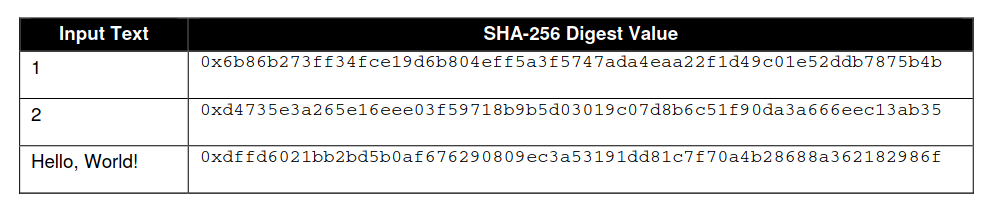
\includegraphics[width=1\textwidth]{images/example_of_sha-256.png}
			\caption[Example input and output of SHA-256 Digest Value]{Example I/O of SHA-256 Digest Value}
			\label{fig:example_of_sha-256}
		\end{figure}

	\bigbreak
	
	\emph{Public/Private Key} -	
	Asymmetric-key cryptography (or public-key cryptography) uses a pair of keys: a public key and a private key that are mathematically related. It could be infeasible to generate one key from the other.
	The private key is kept secret while the public key can be to everyone, both keys are hold inside user's Wallet, which we present in Section~\ref{sec:hd_wallet}.
	One can encrypt with a private key and then decrypt with the public key. 
	Alternately, one can encrypt with a public key and then decrypt with a private key.
	Bitcoin uses asymmetric-key cryptography to digitally sign transactions, verify signatures or in some cases, exchange the key.
	Asymmetric-key cryptography is discussed in Section~\ref{sec:asymmetric_cryptography}.
	Figure~\ref{fig:asymmetric_cryptography} briefly show message exchange usage of the asymmetric protocol.
	
	\begin{figure}[h!]
		\centering
		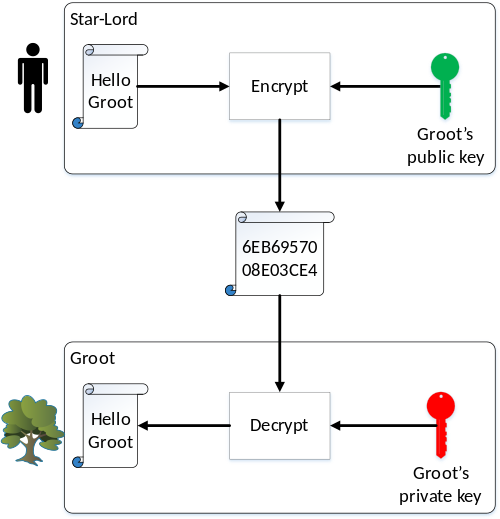
\includegraphics[width=0.4\textwidth]{images/asymmetric_cryptography.png}
		\caption[An example of concept of Asymmetric-key cryptography]{Sending private message using Asymmetric-key cryptography}
		\label{fig:asymmetric_cryptography}
	\end{figure}
	\bigbreak

	\emph{Transactions} - Transactions represent transfers of the cryptocurrencies between wallets in the system. 
	A transaction contains input and output. The inputs are usually a list of the digital assets to be transferred.
	Outputs are	the accounts that will be the recipients of the digital assets along with how much digital asset they will receive.   
	All values of in and out cannot be tampered.

	\begin{figure}[h!]
		\centering
		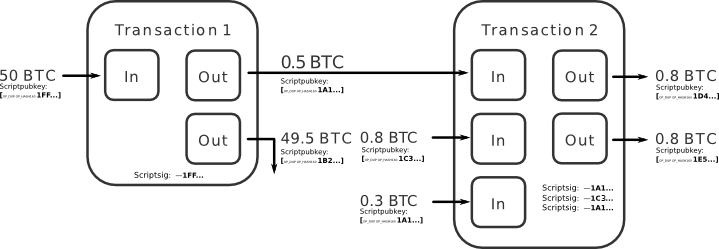
\includegraphics[width=0.7\textwidth]{images/transaction.png}
		\caption[An example of bitcoin transaction]{An example of bitcoin transaction}
		\label{fig:transaction}
	\end{figure}
	\bigbreak

	All transactions are broadcast to the network and usually begin to be confirmed within 10-20 minutes, through a process called \emph{mining}.
	Transactions are typically digitally signed by the sender’s associated private key and can be verified using the associated public key.

	\bigbreak

	\emph{Ledgers} - 
	A ledger is a collection of cryptographic transactions. 
	Bitcoin ledgers are distributed, the blockchain holds all accepted transactions within its ledgers. Every user can maintain their own copy of the ledger.
	Whenever new full nodes join the blockchain network, they reach out to discover other full nodes and request a full copy of the blockchain network’s ledger, making loss or destruction of the ledger difficult.
	\bigbreak
	
	The network utilizes cryptographic mechanisms such as digital signatures and cryptographic hash functions to provide tamper-evident and tamper-resistant ledgers.
	Due to the public distributed network, the Bitcoin blockchain is harder to attack. There is nothing to steal because everything is distributed. If one individual node got taken down, the network will still be running. 
	If targeting the blockchain itself, the attackers will face resistance from the honest nodes present in the system. 
	\bigbreak

	\emph{Blocks} -	
	Transactions, after sent to the network (by wallets, web applications, etc.), will be, if accepted, added to a block that is published by a chosen node. 
	Bitcoin blocks include block header and block data.
	Figure~\ref{fig:block_component} show basic component of a block.
	Block header contains version, previous block header’s hash value (prevBlockHash), a hash representation of the block data (usual Merkle tree* hash), a timestamp, size of the block (bits), a \emph{nonce}.
	The \emph{nonce} value is manipulated by the publishing node to solve the hash puzzle (see Section~\ref{subsec:game_theory})
	Block data contains a list of transactions and ledger events. Some include other data.
	\pagebreak

	\begin{figure}[h!]
		\centering
		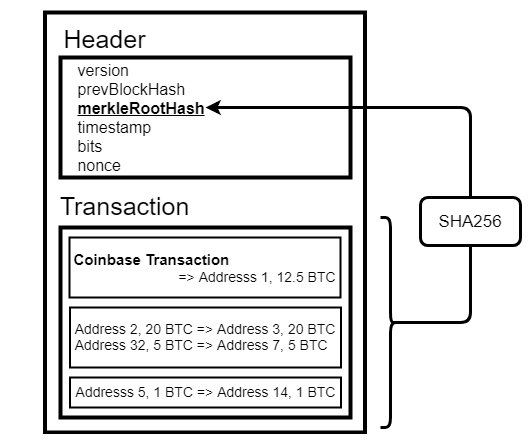
\includegraphics[width=0.6\textwidth]{images/block_component.jpg}
		\caption[Components of Bitcoin block]{Components of Bitcoin block}
		\label{fig:block_component}
	\end{figure}

	\emph{Chain of Blocks} - 
	Blocks are chained together through each block containing the hash digest of the previous block’s header, thus forming the blockchain.
	If one of the previous blocks were changed, it would result in a different hash.
	This makes it possible to easily detect and reject altered blocks

	\begin{figure}[h!]
		\centering
		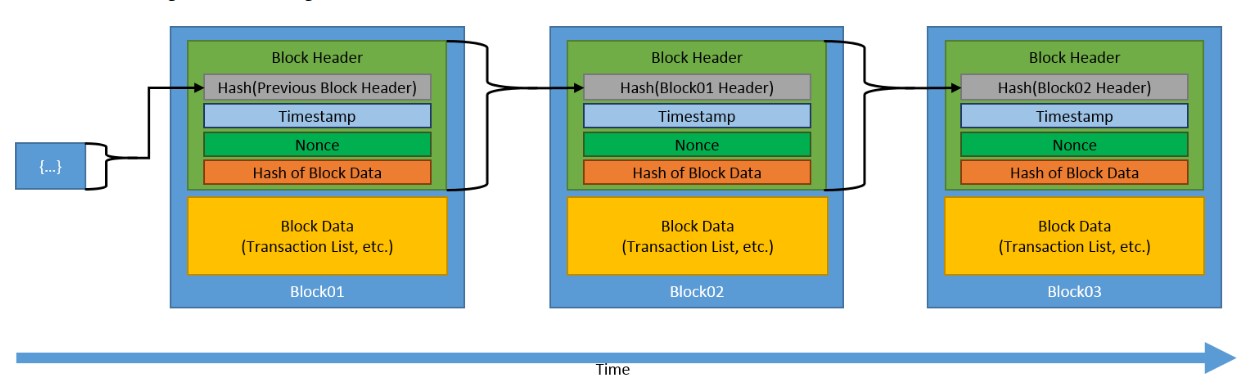
\includegraphics[width=1\textwidth]{images/chain_of_block.png}
		\caption[Components of Bitcoin block]{Components of Bitcoin block}
		\label{fig:chain_of_block}
	\end{figure}


\end{quote}

\item Game of theory and Incentives
\label{subsec:game_theory}

\begin{quote} 
	\emph{Hashes} - 
	Cryptographic hash functions (CHF) are used for hashing the content of a block, validating the integrity of data, reduce the size of the message or keys, generating a Bitcoin address. We will show detail at Section~\ref{sec:crypto_hash}.
	Hashing is a method of calculating a relatively unique fixed-size output (called a message digest, or just digest) for an input of nearly any size (e.g., a file, some text, or an image).
	Even one single bit change of input will result in a completely different output digest. 


\end{quote}
\item Communication Network

\begin{quote} 
	\emph{Hashes} - 
	Cryptographic hash functions (CHF) are used for hashing the content of a block, validating the integrity of data, reduce the size of the message or keys, generating a Bitcoin address. We will show detail at Section~\ref{sec:crypto_hash}.
	Hashing is a method of calculating a relatively unique fixed-size output (called a message digest, or just digest) for an input of nearly any size (e.g., a file, some text, or an image).
	Even one single bit change of input will result in a completely different output digest. 

\end{quote}

\end{itemize}



\section{HDWallet}
\label{sec:hd_wallet}

\subsection{Blockchain wallet}
A blockchain wallet, sometimes referred as a cryptocurrency wallet, is a program that allows you to “store”, send and receive digital currencies. Since cryptocurrency doesn’t exist in any physical form, your wallet doesn’t hold any of your coins actually. Instead, it tracks the transactions you made, which is stored in blockchain, and then infers your balance. Thereby, blockchain is an essential component of a blockchain wallet.

Instead of holding physical coins, a wallet has a public key and a private key. Public key is a long sequence of letters and numbers that forms the wallet address. With this, people can send money to the wallet. It's similar to a bank account number in that it can only be used to send money to an account. Private key is used to access the funds stored in the wallet. With this, people can control the funds tied to that wallet's address. It's a lot like your PIN number in that you should keep it 100\% secret and secure. However, it's worth noting that not all wallets give you sole ownership of your private key, which essentially means that you don't have full control over your coins. As well as storing your public and private keys, crypto wallets interface with the blockchains of various currencies so that you can check your balance and send and receive funds.

\subsection{Category}

Now that you know what is, let’s take a closer look at the five different types of wallets available, each with its own advantages and disadvantages in terms of security, ease of use, convenience and a range of other factors. The most common type of wallet out there, desktop wallets are downloaded and installed on your computer. Easy to set up and maintain, most are available for Windows, Linux and Mac, although some may be limited to a particular operating system. Many cryptocurrencies offer a desktop wallet specifically designed for their coin.

Desktop wallets provide a relatively high level of security since they’re only accessible from the machine on which they’re installed. The biggest disadvantage is that they also rely on you to keep your computer secure and free of malware, so antivirus and anti-malware software, a strong firewall and a common-sense approach to security are required to keep your coins safe. Most desktop wallets will provide you with a long string of words upon installation. These words are known as your recovery seed or sentence and map with your private key, so it’s important to store them somewhere safe in case your computer dies or you need to format the operating system and re-install your desktop wallet. Some popular desktop wallets: Electrum, Exodus, Copay.

Mobile wallets are fairly similar to desktop wallets, with the obvious difference being that they run as an app on your smartphone. Mobile wallets feature many of the same advantages and disadvantages as desktop wallets, with your private key stored on your device.
Smartphone wallets are often easier to use compared to their desktop counterparts and include the ability to scan other wallet addresses for faster transactions. They also make it simpler to access your coins on the go and use cryptocurrency as part of everyday life. You will need to be extra careful about losing your smartphone, though, because there’s a risk that anyone who has access to your device might also have access to your funds. Choosing an app that allows you to back up your wallet with a 12- or 24-word passphrase is a good idea. Popular mobile wallets: Jaxx, Coinomi, Edge.

Online wallets (most often provided by exchanges but sometimes offered by third parties) are connected to the Internet and are generally the easiest to set up and use. Most only require an email address and a password to create an account, and web wallets are usually designed to provide a simple and straightforward user experience. The biggest advantages to online wallets are that they can’t be lost and that they’re accessible from any computer with an Internet connection. However, being online is unfortunately also their biggest disadvantage. Because some platforms maintain the wallets of thousands of users, they can become hot targets for hackers. It’s also important to check whether the wallet you choose lets you retain complete control of your private keys or whether they’re owned by the wallet provider. Popular web wallets: blockchain.info, MyEtherWallet, Coinbase.

Hardware wallets add another layer of security by keeping your private key on a USB stick or specially designed piece of hardware. They allow the user to plug the USB stick into any computer, log in, transact and unplug – so while transactions are carried out online, your private key is stored offline and protected against the risk of hacking. As a result, hardware wallets are widely considered to offer the most secure storage option. The biggest disadvantage of hardware wallets is that they’ll cost you. Prices vary depending on the model you choose, but they generally cost upwards of \$150. You also need to keep the device safe, but if you do lose your hardware wallet, the device itself is PIN-protected and there are usually other protective measures in place to help you recover your funds. Popular hardware wallets: Ledger Nano X, Ledger Nano S, TREZOR, KeepKey.

Paper wallets take the concept of entirely offline keys used for hardware wallets to the next logical step: simply print out your public and private keys and use that piece of paper as your wallet. As secure as they are, paper wallets are also complex and quite confusing for beginners. They’re typically only used by advanced users who want a high level of security. To transfer money to a paper wallet, you use a software wallet (any of the above mentioned) to send money to the public key printed on the sheet of paper. Most often, this is printed as a QR code for easy scanning. To transfer money from the paper wallet to someone else, you would first need to transfer money to a software wallet (by manually entering the private key into the software), and then transfer money from the software wallet to the recipient as usual. Popular paper wallets: Bitaddress.org, WalletGenerator.net.

As you’re researching and comparing a range of wallets, you’ll probably come across the terms “hot wallet” and “cold wallet”, or perhaps the concept of “cold storage”. So, what does temperature have to do with crypto storage?
A wallet is hot when it's connected to the Internet. Nothing on the Internet is 100\% secure, so funds kept in a hot wallet are always at a slight risk of theft or loss from software bugs or hackers. A wallet is cold when it's safely offline and can't be deliberately or accidentally compromised over the Internet.

\subsection{HDWallet}


\section{Cryptography}

\subsection{Cryptographic hash}
\label{sec:crypto_hash}

\subsection{Asymmetric-key cryptography}
\label{sec:asymmetric_cryptography}

\subsubsection{Diffie-Hellman algorithm}

\subsubsection{RSA Cryptography}

\subsubsection{ECC - Elliptic Curve Cryptography}

\subsection{Twisted-Edward curve and Ed25519}

\subsection{Child key derivation function}

\chapter{Methodologies and Approaches} \label{chap:Methodologies_and_Approaches}

There are already a HD wallet for Secp256k1. Fortunately, it's open source and the explanation is clear. We can study how to generate a child key on Secp256k1, then try to apply or adjust the CKD function on Ed25519. The reason why is that both Secp256k1 and Curve25519 (the curve 'used' in Ed25519) share the same form, Montgomery. The differences are:

\begin{itemize}
    \item The curves are defined over distinct fields
    \item Curve25519 is birationally equivalent to Ed25519, not the main curve
    \item Ed25519 is a twisted Edwards curve, while Secp256k1 and Curve25519 are \\ Montgomery curve
\end{itemize}

With that being said, some works on Ed25519 has been done. However; none of them are official. Even NIST is still proposing Ed25519 on draft. That means we have to proove the correctness of the math behind CKD function. This is the most challenging problem. Our plan now is learn about modern cryptography, especially elliptic curve, twisted curve and twisted Edward curve; then we analyze the CKD function of Secp256k1; finally, applied what we have studied to work out the CKD function for Ed25519 with the proof of correctness and implement it into a wallet.
\chapter{Goals} \label{chap:Goals}

% \section{System Architecture}
% \begin{figure}[!b]
% 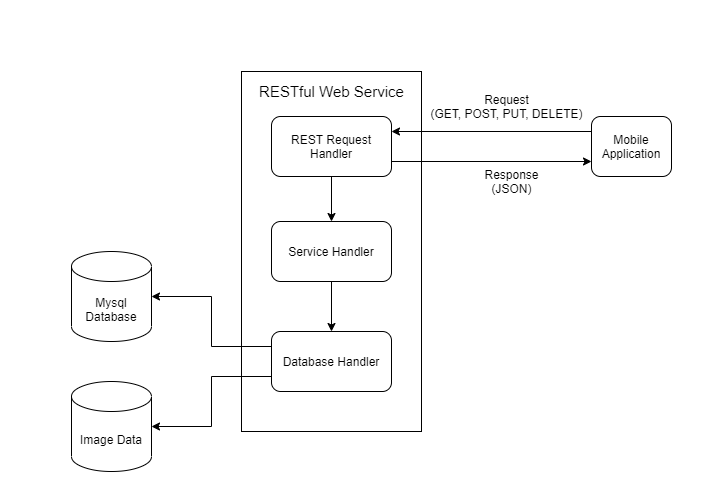
\includegraphics[width=14cm]{Images/App/System_Design.png}
% \caption{System Architecture Design}
% \end{figure}


\chapter{Related works, products and technologies}\label{chap: Related works}

% There are official works on HD wallet for Secp256k1 that we would like to include. First of all is the \emph{BIP0032} \cite{github/bip0032}, a Bitcoin Improvement Proposal that describes hierarchical deterministic wallets. The specification is intended to set a standard for deterministic wallets that can be interchanged between different clients. Although the wallets described here have many features, not all are required by supporting clients. The specification consists of two parts. In a first part, a system for deriving a tree of key pairs from a single seed is presented. The second part demonstrates how to build a wallet structure on top of such a tree. The document explains clearly how they use HMAC-SHA512 to derive a child key. Also, they specify the wallet structure, its use cases and test vector to prove their work. In \cite{DBLP:Deterministic}, their super-wallet/sub-wallet is similar to a master key and a child key. They applied  the \emph{BIP0032} into their model to show a use case of its. However; the model is quite simple and, in a way, separates the master and child key.

% On the other hand, for designing a wallet, there are some works mention about how a wallet is secure and the privacy of blockchain, for instance in \cite{DBLP:towards_blockchain}. They analyzed the wallet and constructs data privacy protection in system. They designed a complete architecture and implementation method of data efficient transaction, such as data three weight separation, data privacy isolation on the chain, cross network and cross cloud deployment algorithm decomposition multi center collaboration, as well as collaborative services on the chain and off the chain, focusing on the feasibility and simple and effective implementation.
\chapter{Conclusion and Future Work} \label{chap:conclusion}

% \section{conclusion}
% The field diagram detection is an interesting and complex study domain. Although there are many research about on-line diagram, there is still less research about recognizing off-line diagram. With this thesis proposal, we have achieved new background knowledge about the computer vision. We are able to access each procedures in image processing which is also a new field for us. We finds many approaches for handwriting flowchart recognition and we select the suitable approaches using Faster R-CNN, YOLO v4 and RefineDet.\\
% During the research process, our group still had many problems in teamwork, lack of time management skills which affects negatively our result. This problems may become a wall in our work in the future, which we need to overcome and improve our working process.

% \section{Challenges}
% \begin{itemize}
%     \item One of the biggest problem with server-client system is scaling or the amount of customers serving at the same time. Most of our experiment is conducted in the local machine so that there is a need to find a way to provide more stable service in the final product.
%     \item The target is to support a wide range of products so as many devices can install this app as possible. Then it can lead to performance issues and the need to find a balance between stable functioning and feature variety.
%     \item Security is also important since many of these data can be very crucial. All of the information sent or receive by the app and the server need to be secured in order to prevent data leak.
% \end{itemize}

% \section{Future work}
% In the future, we are going to implement the flowchart recognition system and also evaluate the capabilities of the programming languages and the support framework to reduce the constraints of our proposed system while solving all of the listed challenges.

\renewcommand{\bibname}{References}
\bibliography{refs}
\bibliographystyle{unsrt}


\end{document}
